\section{Presentation Logic Layer}

%What pages will be present in your project? briefly indicate how your web site will be organized

The website will be divided into the following pages:
\begin{itemize}
    \item Homepage: contains the showcase of the avaible products. Written in jsp.
    \item Product page: allows the customer to buy the products he is looking for. Must be logged in.
    \item Login page: allows both the customer and the various employees login to the web application. 
    \item User edit page: both customer and employee are able to modify their personal data using a simple form. 
    \item Order list and Order details page: allows each customer to look at their order history to open a ticket, cancel the order or get the invoice.
    \item Tickets page: allows each customer to look at their ticket history. Exists an employee version of the page that allows to manage each ticket.
    \item Product management pages: both simple employees and administrators are able to look at all the products and edit/delete them. Through a second page (Discount management) is also possible to add some discounts.
    \item Orders management page: both simple employees and administrators are able to look at all the orders and edit/cancel them. It's also possible to look at the existing invoices for each product.
    \item Administration page: allows the administrators to edit the roles of all the users and even delete their account.
\end{itemize}

\subsection{Homepage}
    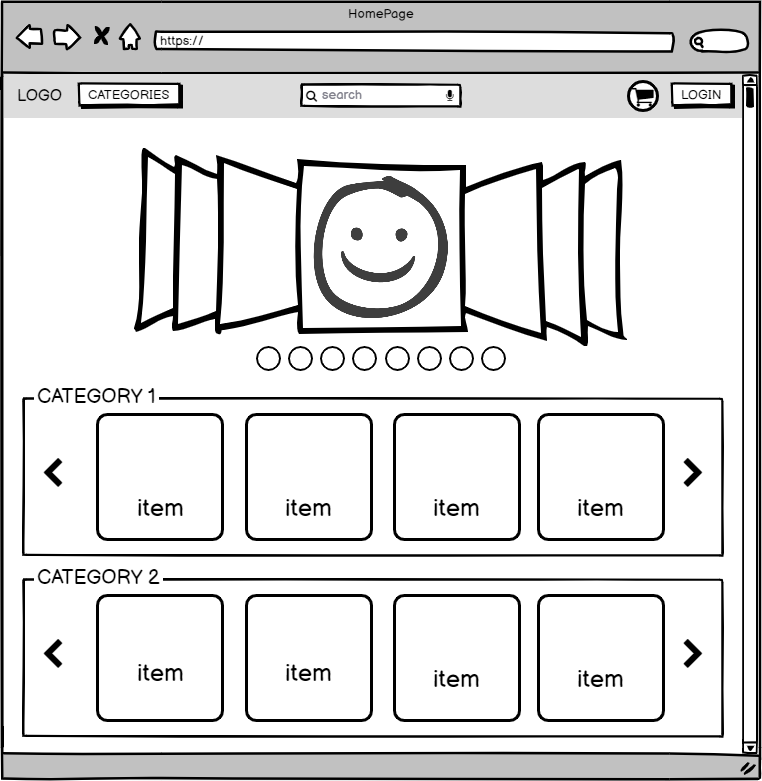
\includegraphics[width=\textwidth,height=\textheight,keepaspectratio]{mockups/homepageMockup.png}

The homepage contains the main information regarding the various products available.
The products are divided into sessions according to their category.This subdivision will be done by means of a scrollable list. Moreover, the homepage contains a bar to search by name of the single elements.
Like most of the top pages, the homepage contains a status bar that allows the user to register, log in or log out once logged in.
Finally, this status bar allows customers to show the history of the products purchased.

\subsection{Product page}
    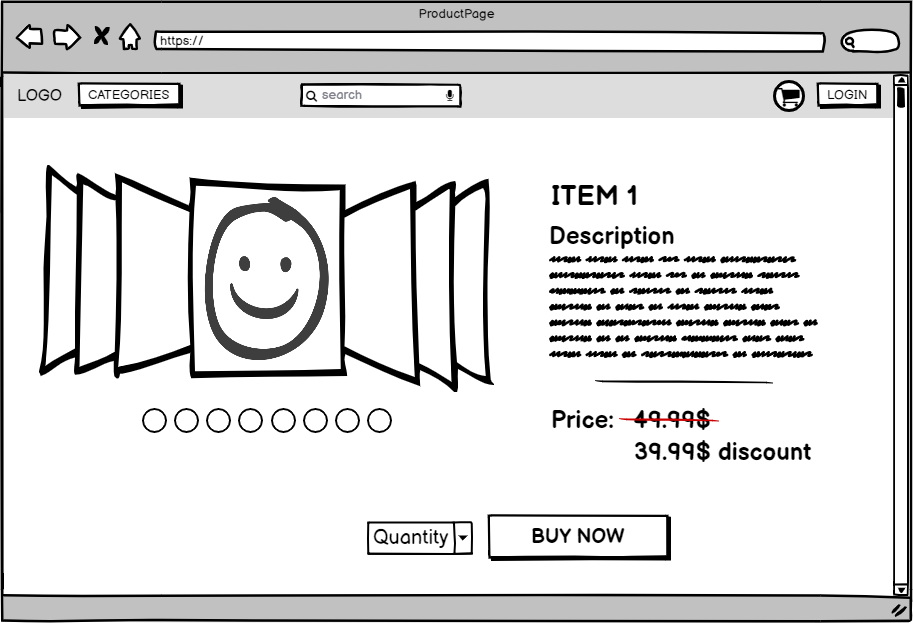
\includegraphics[width=\textwidth,height=\textheight,keepaspectratio]{mockups/productPageMockup.png}

The product page shows in detail the information regarding the individual product.
This page shows all the photos available for a given product, the description and the price.
In addition, it also shows any discount applied to the product.
If the customer is logged in, it will be possible for him to purchase the product within the maximum quantity available. It is possible to enter these particular pages by clicking on the product on the homepage or by searching by product name.

\subsection{UserEdit page}
    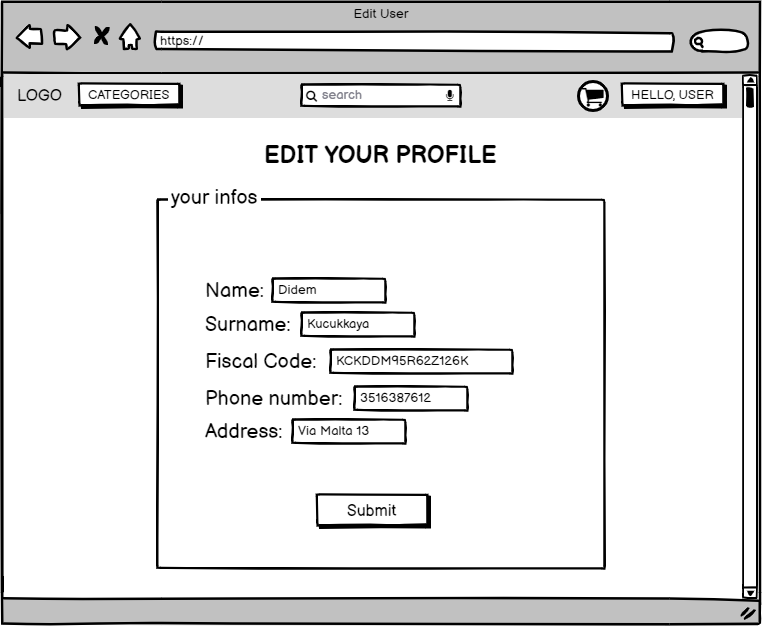
\includegraphics[width=\textwidth,height=\textheight,keepaspectratio]{mockups/userEditPageMockup.png}

The user edit page allows the customer type user to change their personal data.The page will consist of text boxes with default values ​​corresponding to the values ​​previously entered by the user. The page allows you to change data such as telephone number, name, surname but not unique / primary key data. This is because these particular data are used for login, and to avoid conflicts it was decided to do so.
Obviously this page will be available only after the user login.

\subsection{OrderList and OrderDetails}
    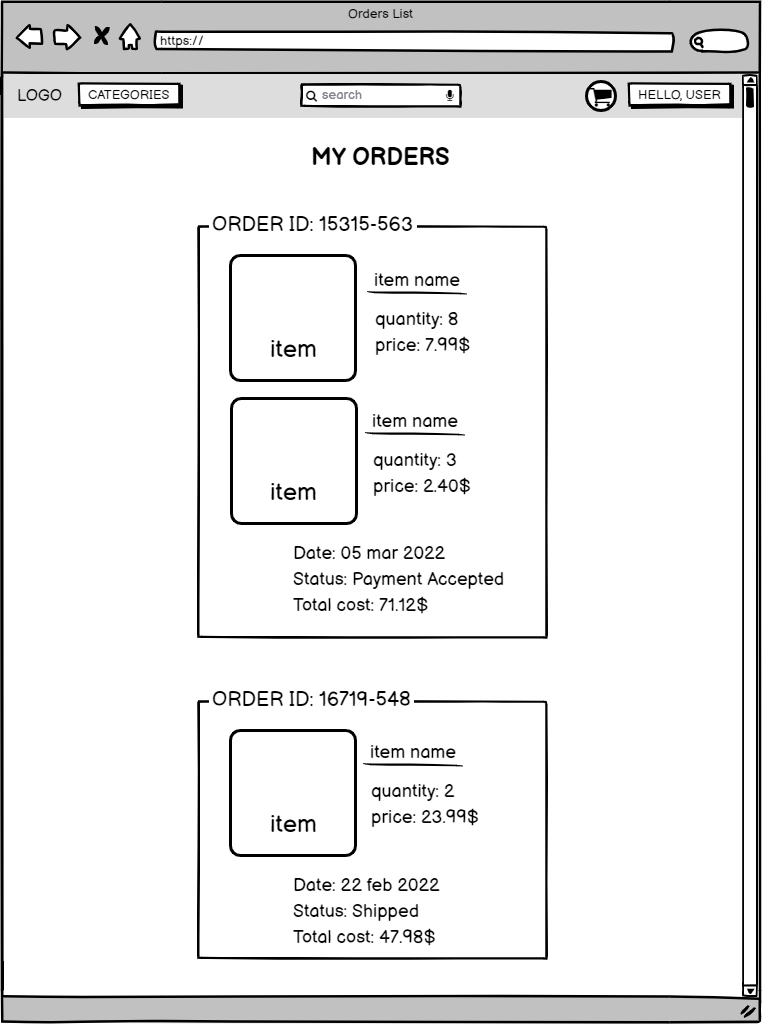
\includegraphics[width=\textwidth,height=\textheight,keepaspectratio]{mockups/ordersPageMockup.png}

    Lorem ipsum dolor sit amet, consectetur adipiscing elit, sed do eiusmod tempor incididunt ut labore et dolore magna aliqua. Ut enim ad minim veniam, quis nostrud exercitation ullamco laboris nisi ut aliquip ex ea commodo consequat. Duis aute irure dolor in reprehenderit in voluptate velit esse cillum dolore eu fugiat nulla pariatur. Excepteur sint occaecat cupidatat non proident, sunt in culpa qui officia deserunt mollit anim id est laborum.


\subsection{Admin: product management}
    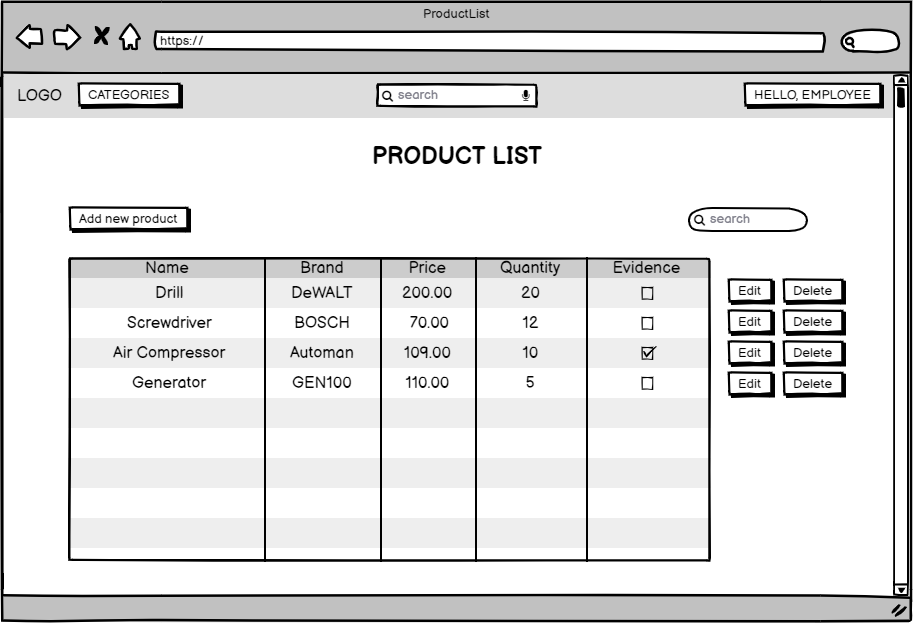
\includegraphics[width=\textwidth,height=\textheight,keepaspectratio]{mockups/productListPageMockup.png}
    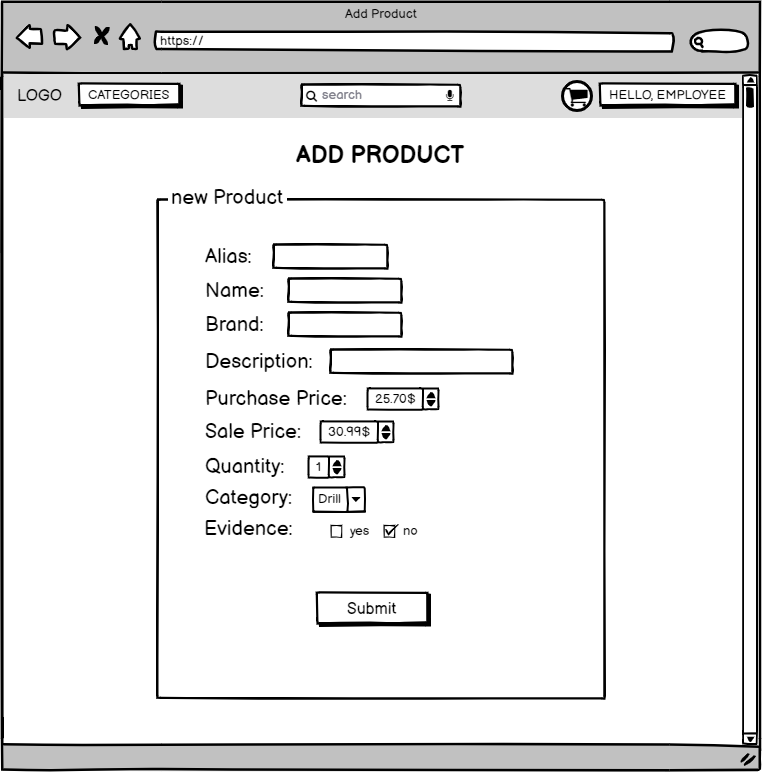
\includegraphics[width=\textwidth,height=\textheight,keepaspectratio]{mockups/addProductPageMockup.png}

    Lorem ipsum dolor sit amet, consectetur adipiscing elit, sed do eiusmod tempor incididunt ut labore et dolore magna aliqua. Ut enim ad minim veniam, quis nostrud exercitation ullamco laboris nisi ut aliquip ex ea commodo consequat. Duis aute irure dolor in reprehenderit in voluptate velit esse cillum dolore eu fugiat nulla pariatur. Excepteur sint occaecat cupidatat non proident, sunt in culpa qui officia deserunt mollit anim id est laborum.


\subsection{Admin: user management}
    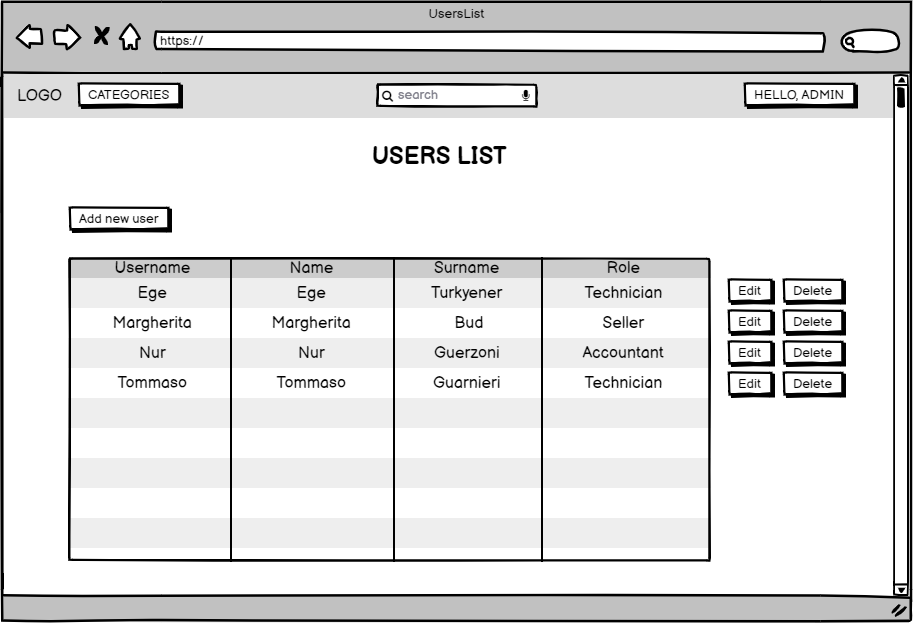
\includegraphics[width=\textwidth,height=\textheight,keepaspectratio]{mockups/usersListPageMockup.png}

    Lorem ipsum dolor sit amet, consectetur adipiscing elit, sed do eiusmod tempor incididunt ut labore et dolore magna aliqua. Ut enim ad minim veniam, quis nostrud exercitation ullamco laboris nisi ut aliquip ex ea commodo consequat. Duis aute irure dolor in reprehenderit in voluptate velit esse cillum dolore eu fugiat nulla pariatur. Excepteur sint occaecat cupidatat non proident, sunt in culpa qui officia deserunt mollit anim id est laborum.

\subsection{Ticket list management}
    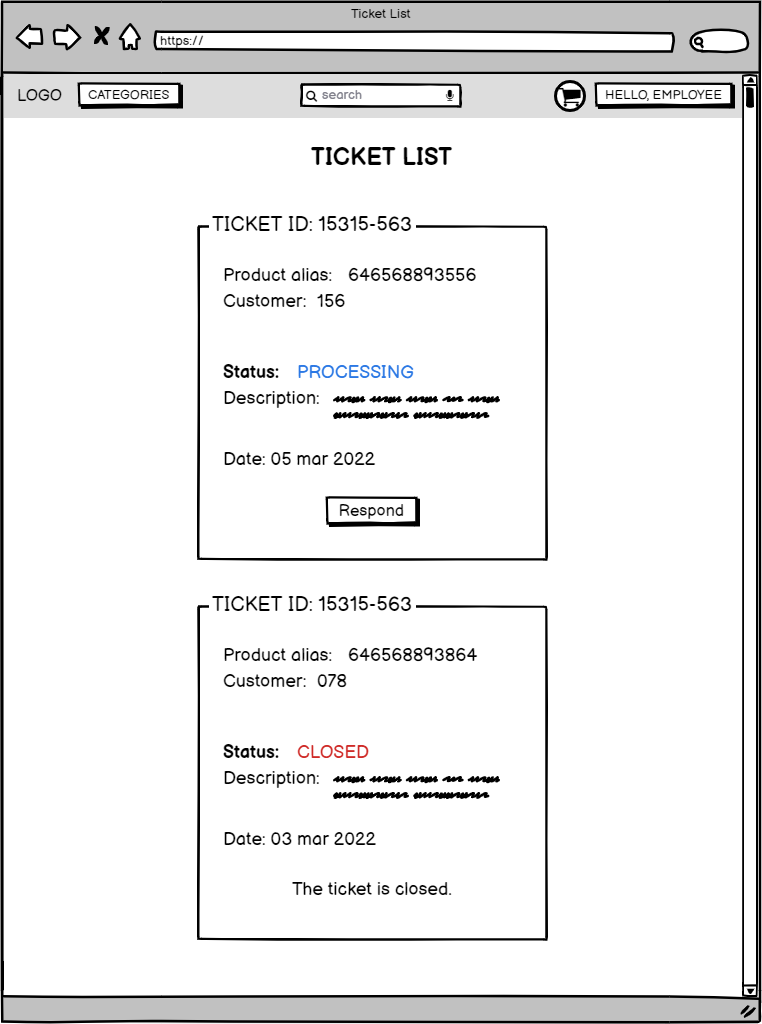
\includegraphics[width=\textwidth,height=\textheight,keepaspectratio]{mockups/ticketPageMockup.png}

    Lorem ipsum dolor sit amet, consectetur adipiscing elit, sed do eiusmod tempor incididunt ut labore et dolore magna aliqua. Ut enim ad minim veniam, quis nostrud exercitation ullamco laboris nisi ut aliquip ex ea commodo consequat. Duis aute irure dolor in reprehenderit in voluptate velit esse cillum dolore eu fugiat nulla pariatur. Excepteur sint occaecat cupidatat non proident, sunt in culpa qui officia deserunt mollit anim id est laborum.

